\section{Context Diagram}

Since the proposed system falls into the category of an open system, it communicates with a lot of external parties. It's advised to have a clear system boundary when developing such a system so the development process doesn't get overwhelming. Figure \ref{fig:context-digram} explain the main interactions between the system and the third parties.

\begin{figure}[H]
    % \setlength{\fboxsep}{10pt}
   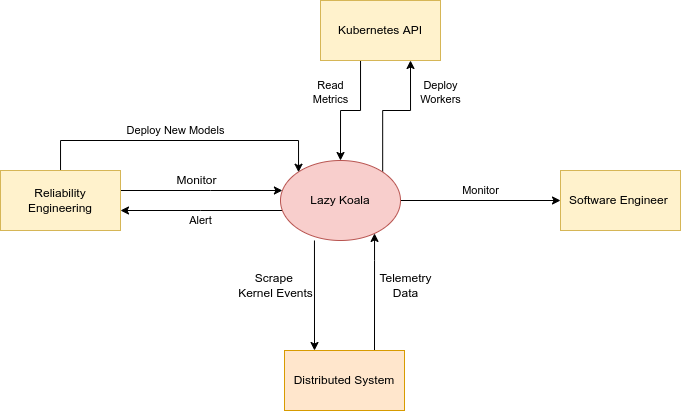
\includegraphics[width=13cm]{assets/requirement-specification/contex-digram.png}
    \caption{Context diagram (self-composed)}
    \label{fig:context-digram}
\end{figure}
